% CPU/GPU correlation
GPUs are usually used in a heterogeneous model containing two different processors, namely the CPU and the GPU as presented on \cref{fig:hw-cpu-gpu}.
The configuration of this CPU/GPU architecture comes in different varieties, however, the variant with one CPU communicating with one GPU is the most common.
Here, the CPU is responsible of executing code on the GPU as well manage the GPUs memory.

\begin{figure}[ht]
	\centering
	\fbox{
		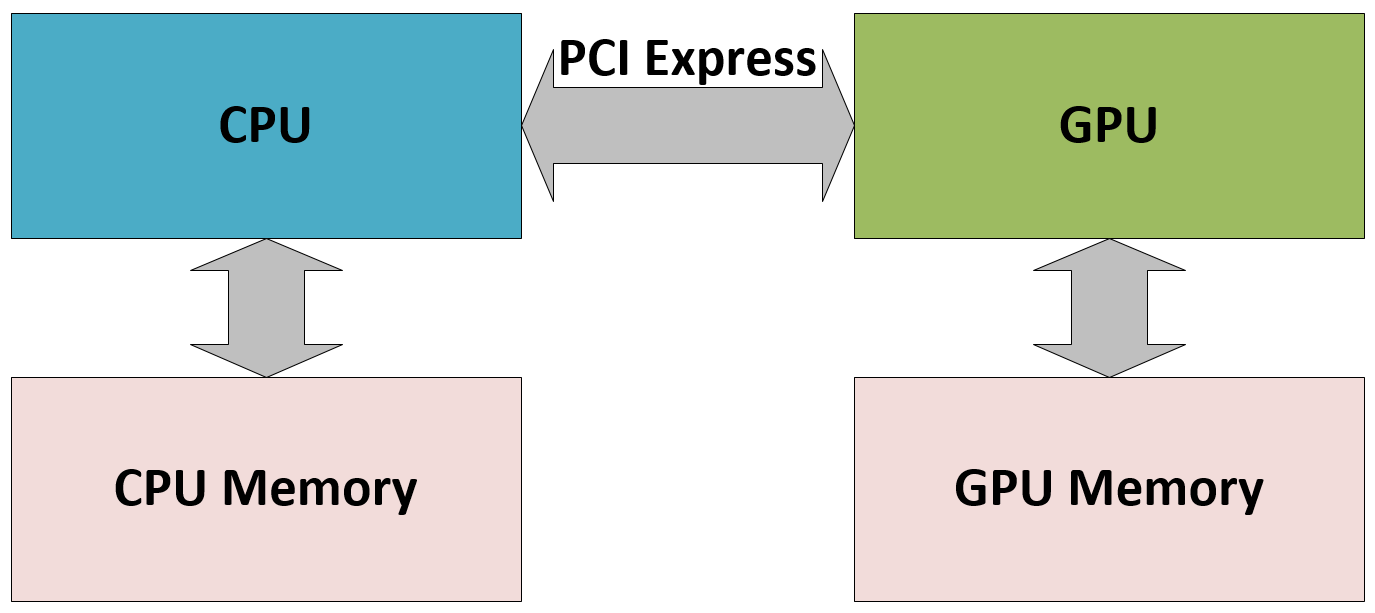
\includegraphics[width=0.8\textwidth]{figs/hw/hw-cpu-gpu}}
	\caption{CPU/GPU architecture}
	\label{fig:hw-cpu-gpu}
\end{figure}

%TODO Add more? Sandybridge!?

%Shane Cook: SandyBridge
%From the I7/X58 chipset design, Intel moved onto the Sandybridge design, shown in Figure 3.3.
%One of the most noticeable improvements was the support for the SATA-3 standard, which supports
%600 MB/s transfer rates. This, combined with SSDs, allows for considerable input/output (I/O)
%performance with loading and saving data.
%The other major advance with the Sandybridge design was the introduction of the AVX (Advanced
%Vector Extensions) instruction set, also supported by AMD processors. AVX allows for vector
%instructions that provide up to four double-precision (256 bit/32 byte) wide vector operations. It’s
%a very interesting development and something that can be used to considerably speed up computebound
%applications on the CPU.









